\documentclass[preprint,12pt,3p]{elsarticle}
\usepackage{amsmath,amssymb,amsthm,mathtools}
\usepackage{float,algpseudocode}
\newfloat{algorithm}{htbp}{loa}
\floatname{algorithm}{Algorithm}
\usepackage{graphicx,booktabs,longtable,xcolor}
\usepackage[bookmarks=false]{hyperref}
\usepackage{cleveref}
\journal{Journal of Computational and Applied Mathematics}
\newtheorem{theorem}{Theorem}[section]
\newtheorem{lemma}[theorem]{Lemma}
\newtheorem{proposition}[theorem]{Proposition}
\theoremstyle{definition}
\newtheorem{definition}[theorem]{Definition}
\newtheorem{assumption}[theorem]{Assumption}
\newtheorem{remark}[theorem]{Remark}
\newtheorem{example}[theorem]{Example}
\DeclareMathOperator*{\argmin}{arg\,min}
\DeclareMathOperator{\Fix}{Fix}
\DeclareMathOperator{\Id}{Id}
\DeclareMathOperator{\zer}{zer}
\newif\ifchanges
\changesfalse
\makeatletter
\renewcommand{\theALG@line}{\thealgorithm.\arabic{ALG@line}}
\providecommand{\theHALG@line}{}
\renewcommand{\theHALG@line}{\thealgorithm.\arabic{ALG@line}}
\makeatother
\makeatletter
\pdfstringdefDisableCommands{%
  \def\cnotenum{}%
  \let\@corref\@gobble
  \let\corref\@gobble
  \let\ead\@gobble
}
\makeatother
% ===== Begin inlined file: numbers.tex =====
\newcommand{\NumRunCount}{45}
\newcommand{\NumInstanceCount}{15}
\newcommand{\NumCertifiedRunCount}{30}
\newcommand{\NumHybridOverheadTwenty}{41.42}
\newcommand{\NumHybridSpeedupFifty}{11.31}
\newcommand{\NumHybridSpeedupHundred}{17.90}
\newcommand{\NumHybridSpeedupMin}{-74.16}
\newcommand{\NumHybridSpeedupMax}{19.87}
\newcommand{\NumMaxCertifiedAbsGap}{8.089959}
\newcommand{\NumMaxCertifiedRelGapPct}{0.000346}
\newcommand{\NumMLResidualMin}{2.282}
\newcommand{\NumMLResidualMax}{8.181}
\newcommand{\NumValidationMeanMW}{5.657}
\expandafter\newcommand\csname NumValidationP90MW\endcsname{9.683}
\newcommand{\NumOfflineWall}{79.33}
\newcommand{\NumDatagenWall}{45.66}
\newcommand{\NumTrainingWall}{33.67}
\newcommand{\NumWorstInnerResidual}{1.392\times 10^{-6}}
\newcommand{\NumWorstInnerMu}{1.127\times 10^{-7}}
\newcommand{\NumWorstInnerIterations}{48}
\newcommand{\NumMaxDualPrimalSpread}{0.007216}
\newcommand{\NumMaxPinnedPrimalDualSpread}{0.006737}
\newcommand{\NumHybridSpeedupMinTwenty}{-74.16}
\newcommand{\NumHybridSpeedupMaxTwenty}{-25.30}
\newcommand{\NumHybridSpeedupMedianTwenty}{-41.42}
\newcommand{\NumHybridFasterCountTwenty}{0}
\newcommand{\NumHybridSlowerCountTwenty}{5}
\newcommand{\NumHybridSpeedupMinFifty}{11.31}
\newcommand{\NumHybridSpeedupMaxFifty}{16.10}
\newcommand{\NumHybridSpeedupMedianFifty}{14.74}
\newcommand{\NumHybridFasterCountFifty}{5}
\newcommand{\NumHybridSlowerCountFifty}{0}
\newcommand{\NumHybridSpeedupMinHundred}{12.12}
\newcommand{\NumHybridSpeedupMaxHundred}{19.87}
\newcommand{\NumHybridSpeedupMedianHundred}{18.06}
\newcommand{\NumHybridFasterCountHundred}{5}
\newcommand{\NumHybridSlowerCountHundred}{0}
\newcommand{\NumIORetryCount}{10}
% ===== End inlined file: numbers.tex =====
\newcommand{\Num}[1]{\csname Num#1\endcsname}
\setlength{\emergencystretch}{1em}
% The elsarticle front-matter output box has a fixed 2.608 pt overhang;
% page-level PDF inspection confirms that it is not clipped.
\setlength{\hfuzz}{3pt}

\begin{document}
\ifchanges\color{blue}\fi
\begin{frontmatter}
\title{Learning-Accelerated ADMM: Convergence Theory and Application to Stochastic Optimal Power Flow}
\author[1]{Yonghong Yao}\ead{yyhtgu@hotmail.com}
\author[2]{Yekini Shehu\corref{cor1}}\ead{yekini.shehu@zjnu.edu.cn}
\cortext[cor1]{Corresponding author}
\address[1]{School of Mathematical Sciences, Tiangong University, Tianjin 300387, China; and Department of Medical Research, China Medical University Hospital, China Medical University, Taichung, Taiwan.}
\address[2]{School of Mathematical Sciences, Zhejiang Normal University, Jinhua 321004, China}
\begin{abstract}
We study scenario-consensus ADMM in which a recurrent neural network predicts only the initial recourse block. The learned update is treated as an inexact Douglas--Rachford step. Under summable realized block errors, the DRS state and the learned initial blocks converge to optimal limiting objects. No full learned recourse vector is assumed to exist. A fixed proxy is not claimed to satisfy this hypothesis. In a region where the DRS operator is contractive and trapping holds, bounded errors give an explicit ultimate-distance bound; outside such a region no plateau theorem is asserted. Global linear convergence is proved only when the partial recourse value function is strongly convex and smooth. A counterexample shows that strong convexity with constraint indicators does not imply global contraction; the previous global polyhedral-QP and inexact activity-identification claims are removed. An exact tail gives convergence from any learned warm start. Finite termination is evaluated separately by primal/dual residuals, a scenario-dual lower bound, and an independently solved pinned-recourse upper value. In $\Num{RunCount}$ fully regenerated cold-solve runs on an elastic IEEE 118-bus DC-OPF model, all $\Num{CertifiedRunCount}$ exact and hybrid runs meet both $10^{-4}$ residual tolerances. Over five paired seeds per scenario count, signed hybrid speedups range from $\Num{HybridSpeedupMinTwenty}\%$ to $\Num{HybridSpeedupMaxTwenty}\%$ at $S=20$, from $\Num{HybridSpeedupMinFifty}\%$ to $\Num{HybridSpeedupMaxFifty}\%$ at $S=50$, and from $\Num{HybridSpeedupMinHundred}\%$ to $\Num{HybridSpeedupMaxHundred}\%$ at $S=100$. The fixed proxy stalls with consensus residuals $\Num{MLResidualMin}$--$\Num{MLResidualMax}$ MW and is not certified. All legacy and synthetic numerical records are excluded; raw states, certificates, source hashes, and independent replay checks accompany the paper.
\end{abstract}
\begin{keyword}
ADMM \sep Douglas--Rachford splitting \sep inexact proximal algorithms \sep learning to optimize \sep stochastic optimal power flow
\end{keyword}
\end{frontmatter}

% ===== Begin inlined file: sections/introduction.tex =====
\section{Introduction}
Two-stage stochastic programming provides a common here-and-now decision together with scenario-dependent recourse decisions \cite{birge2011introduction,shapiro2009lectures}. Scenario-consensus ADMM, closely related to progressive hedging \cite{rockafellar1991scenarios}, replaces a centralized solve by repeated scenario subproblems \cite{eckstein1992douglas,boyd2011distributed}. This decomposition is useful when the scenario subproblems are tractable, but their repeated solution remains the dominant cost in the present multi-period OPF application.

Learning to optimize offers a possible way to amortize that cost by predicting optimization maps or warm starts \cite{chen2022learning,amos2023tutorial,sambharya2024learning}. A learned proximal map, however, is not automatically an accurate one. Replacing an exact scenario update changes the fixed-point recursion, and feasibility of a predicted initial block does not imply either optimality or feasibility of a complete recourse trajectory. The central distinction in this paper is therefore between a heuristic fixed-proxy iteration, a conditional inexact method whose realized errors are summable, and a hybrid method with an exact tail. The three must not share the same convergence claim.

Our contributions are deliberately restricted to statements supported by proof or regenerated evidence.
\begin{enumerate}
\item We give an initial-block formulation of learned scenario-consensus ADMM and derive its DRS error recursion in the probability-weighted metric. Full-recourse statements are made only for exact subproblem solutions.
\item We prove convergence under summable realized errors and a trapping-neighborhood bound under explicitly assumed contraction and entry hypotheses. Global linear convergence is proved only for a strongly convex and smooth partial value function on the entire DRS space. A counterexample delimits this result; contraction is not inferred from residual plots.
\item We derive the per-scenario sensitivity factor and correct the scenario-penalty scaling. Keeping $\rho S$ fixed requires $\rho\propto S^{-1}$; no general $S$-independent contraction factor is claimed for the constrained application.
\item We separate asymptotic convergence from finite-run evidence. The latter combines the standard residual test with a Lagrangian lower bound and an independently solved pinned-recourse value. Appendix~\ref{app:certificates} gives the QP dual and period-zero elimination used to evaluate these bounds. Absolute gaps and solver diagnostics are retained even when relative gaps are unavailable.
\item We release a deterministic numerical study with an expanded scenario-count and seed grid. Every table and figure is generated from raw logs that pass hash, residual, ML-phase identity, exact-tail replay, and certificate-replay checks. Unfavourable timing and fixed-proxy outcomes are reported.
\end{enumerate}

The operator tools used here are classical. The contribution is not a new splitting operator or a universal acceleration theorem; it is a problem-specific framework that identifies precisely what an initial-block learned update can and cannot certify, combines it with computable finite-run lower/upper bounds for the elastic multi-period OPF, and tests those distinctions under a fully replayable protocol. This scope is narrower than the earlier version but is supported by the stated proofs and artifacts.

The paper is organized as follows. Section 2 derives the consensus-ADMM/DRS correspondence. Section 3 analyzes learned initial-block errors. Section 4 specifies the proxy, data generation, exact-tail algorithm, and finite-run bounds. Section 5 states the implemented OPF model, Section 6 reports the regenerated study, and the appendices collect certificate algebra, solver structure, and reproducibility details.

\paragraph{Notation} For $u=(u_1,\ldots,u_S)$ with $u_s\in\mathbb R^n$, define
\[
\langle u,v\rangle_\pi=\sum_{s=1}^S\pi_s\langle u_s,v_s\rangle,\qquad
\|u\|_\pi^2=\sum_{s=1}^S\pi_s\|u_s\|^2,\qquad \pi_s=1/S.
\]
The exact recourse minimizer is $z_s^{k+1}$, its initial block is $z_{s,0}^{k+1}$, and the learned/restored initial block is $\widehat z_{s,0}^{k+1}$. The implemented method forms no learned full vector $\widehat z_s^{k+1}$. Table~\ref{tab:notation} fixes the remaining notation.

\begin{table}[htbp]
\centering
\caption{Notation used in the theory and implementation.}
\label{tab:notation}
\small
\begin{tabular}{ll}
\toprule
Symbol & Meaning\\
\midrule
$x^k$ & first-stage consensus iterate\\
$z_s^{k+1}$ & exact scenario minimizer; $z_{s,0}^{k+1}$ is its initial block\\
$z_s^\star,z_s^\star(x)$ & optimal recourse vector; the latter is pinned to initial block $x$\\
$\widetilde z_{s,0}^{k+1}$ & raw neural-network output\\
$\widehat z_{s,0}^{k+1}$ & restored initial block used by the learned update\\
$\delta_{s,0}^k$ & $\widehat z_{s,0}^{k+1}-z_{s,0}^{k+1}$; $\delta^k=\max_s\|\delta_{s,0}^k\|$\\
$\lambda_s^k$ & multiplier for $x=z_{s,0}$\\
$r^k,s^k$ & max-scenario primal residual and Euclidean dual residual\\
$r_\pi^k$ & probability-weighted consensus residual\\
$u^k,T$ & DRS state and Douglas--Rachford operator\\
$\theta_s,\Theta$ & partial recourse value functions; $\Theta=\sum_s\pi_s\theta_s$\\
$\rho$ & ADMM penalty; the resolvent weight is $t=\rho S$\\
$q(\lambda),V(x)$ & Lagrangian lower bound and pinned-recourse value\\
\bottomrule
\end{tabular}
\end{table}
% ===== End inlined file: sections/introduction.tex =====
% ===== Begin inlined file: sections/admm_drs.tex =====
\section{Consensus ADMM and Douglas--Rachford splitting}
\subsection{Two-stage model}
Consider
\begin{align}
\min_{x,\{z_s\}}\quad &\sum_{s=1}^S\pi_s f_s(z_s)\nonumber\\
\mathrm{s.t.}\quad &z_s\in Z_s,\qquad z_{s,0}=x\quad(s=1,\ldots,S),\qquad x\in X_0,
\label{eq:twostage}
\end{align}
where $X_0$ and each $Z_s$ are nonempty closed convex sets and each $f_s$ is proper closed convex. The partial value functions are
\[
\theta_s(v)=\inf\{f_s(z_s):z_s\in Z_s,\ z_{s,0}=v\},\qquad
\Theta(u)=\sum_{s=1}^S\pi_s\theta_s(u_s).
\]
We assume that $\Theta$ is proper closed convex, that all required scenario minimizers exist, and that \eqref{eq:twostage} has a saddle point. These are standing hypotheses, not consequences of convexity alone.

The augmented Lagrangian is
\[
L_\rho=\iota_{X_0}(x)+\sum_s\left[\pi_s f_s(z_s)+\lambda_s^\top(x-z_{s,0})+\frac{\rho}{2}\|x-z_{s,0}\|^2\right].
\]
With $\alpha=1$, exact consensus ADMM is
\begin{align}
x^{k+1}&=\argmin_{x\in X_0}\sum_s\left[\lambda_s^{k\top}x+\frac{\rho}{2}\|x-z_{s,0}^k\|^2\right],\label{eq:admmx}\\
z_s^{k+1}&=\argmin_{z_s\in Z_s}\left\{\pi_s f_s(z_s)+\lambda_s^{k\top}(x^{k+1}-z_{s,0})+\frac{\rho}{2}\|x^{k+1}-z_{s,0}\|^2\right\},\label{eq:admmz}\\
\lambda_s^{k+1}&=\lambda_s^k+\rho(x^{k+1}-z_{s,0}^{k+1}).\label{eq:admmlam}
\end{align}
For a box $X_0$, \eqref{eq:admmx} is clipping of $\sum_s\pi_s(z_{s,0}^k-\lambda_s^k/\rho)$. The stopping residuals used in every run are
\begin{equation}
r^k=\max_s\|x^k-z_{s,0}^k\|,\qquad
s^k=\rho\|x^k-x^{k-1}\|,\qquad
r_\pi^k=\left(\sum_s\pi_s\|x^k-z_{s,0}^k\|^2\right)^{1/2}.
\label{eq:residuals}
\end{equation}
Both $r^K\leq10^{-4}$ and $s^K\leq10^{-4}$ are required for exact and hybrid termination.

\subsection{DRS correspondence in the weighted metric}
Let $U=(\mathbb R^n)^S$, $\widetilde C=\{u\in U:u_1=\cdots=u_S=x\in X_0\}$, $A=N_{\widetilde C}$, and $B=\partial\Theta$. Both operators are maximal monotone in the $\pi$-inner product. For $t>0$, write $J_{B/t}=(\mathrm{Id}+B/t)^{-1}$ and $R_{B/t}=2J_{B/t}-\mathrm{Id}$, and analogously for $A$. The resolvent $b=J_{B/t}(u)$ is blockwise the initial block of
\begin{equation}
\argmin_{z_s\in Z_s}\left\{f_s(z_s)+\frac{t}{2}\|z_{s,0}-u_s\|^2\right\}.
\label{eq:resolvent}
\end{equation}
Indeed, the block of $\partial\Theta$ associated with the $\pi$-metric is $\partial\theta_s$, so the factor $\pi_s$ cancels from the resolvent optimality condition. Moreover,
\begin{equation}
J_{A/t}(u)=\operatorname{Proj}_{\widetilde C}(u),\qquad
(\operatorname{Proj}_{\widetilde C}(u))_s=\operatorname{Proj}_{X_0}\left(\sum_{j=1}^S\pi_j u_j\right).
\label{eq:consensusproj}
\end{equation}

\begin{lemma}[ADMM--DRS correspondence]\label{lem:admm-drs}
Set $t=\rho S$ and
\[
u_s^k=x^{k+1}+\lambda_s^k/\rho,\qquad b^k=J_{B/t}u^k,\qquad a^k=\operatorname{Proj}_{\widetilde C}(2b^k-u^k).
\]
Then $b_s^k=z_{s,0}^{k+1}$, the common value of $a^k$ is $x^{k+2}$, and exact ADMM \eqref{eq:admmx}--\eqref{eq:admmlam} satisfies
\begin{equation}
u^{k+1}=u^k+a^k-b^k=Tu^k,\qquad T=\tfrac12(\mathrm{Id}+R_{A/t}R_{B/t}),
\label{eq:drs}
\end{equation}
together with $\lambda_s^{k+1}=\rho(u_s^{k+1}-x^{k+2})$. The operator $T$ is firmly nonexpansive in $\|\cdot\|_\pi$, and
\begin{equation}
J_{B/t}(\operatorname{Fix}T)=\operatorname{zer}(A+B).
\label{eq:fixzer}
\end{equation}
\end{lemma}
\begin{proof}
Completing the square in \eqref{eq:admmz} gives
\[
\lambda_s^{k\top}(x^{k+1}-z_{s,0})+\frac{\rho}{2}\|x^{k+1}-z_{s,0}\|^2
=\frac{\rho}{2}\|z_{s,0}-u_s^k\|^2+\text{constant}.
\]
Since $\pi_s=1/S$, the scenario objective in \eqref{eq:admmz} is therefore $\pi_s$ times \eqref{eq:resolvent} with $t=\rho S$, up to a constant. This proves $b_s^k=z_{s,0}^{k+1}$.

By \eqref{eq:consensusproj}, the common value of $a^k$ is the projection onto $X_0$ of
\[
\sum_s\pi_s(2z_{s,0}^{k+1}-x^{k+1}-\lambda_s^k/\rho).
\]
On the other hand, the next ADMM $x$-update is the projection onto $X_0$ of $\sum_s\pi_s(z_{s,0}^{k+1}-\lambda_s^{k+1}/\rho)$. Substitution of \eqref{eq:admmlam} shows that these two arguments are identical, so the common value of $a^k$ is $x^{k+2}$. The formula $u^{k+1}=u^k+a^k-b^k$ is precisely the reflected-resolvent average in \eqref{eq:drs}. Finally,
\[
\rho(u_s^{k+1}-x^{k+2})=\rho(u_s^k-z_{s,0}^{k+1})
=\lambda_s^k+\rho(x^{k+1}-z_{s,0}^{k+1})=\lambda_s^{k+1}.
\]
Firm nonexpansiveness is the standard reflected-resolvent property \cite{eckstein1992douglas,eckstein2015understanding}. If $u^\star=Tu^\star$, then $a^\star=b^\star=:z^\star$; the resolvent optimality conditions give $tz^\star\in tu^\star-Bz^\star$ and $tz^\star\in2tb^\star-tu^\star-Az^\star$, and subtraction yields $0\in Az^\star+Bz^\star$. Conversely, any $z^\star\in\operatorname{zer}(A+B)$ can be represented this way, which proves \eqref{eq:fixzer}.
\end{proof}
The set $\operatorname{Fix}T$ itself need not be a singleton. Firm nonexpansiveness will be used in the equivalent form
\begin{equation}
\|Tu-Tv\|_\pi^2\leq\|u-v\|_\pi^2-\|(\mathrm{Id}-T)u-(\mathrm{Id}-T)v\|_\pi^2.
\label{eq:fne}
\end{equation}
% ===== End inlined file: sections/admm_drs.tex =====
% ===== Begin inlined file: sections/theory.tex =====
\section{Initial-block learned updates and convergence}
\subsection{Feasibility restoration and realized error}
A recurrent proxy $\Phi_\theta$ produces $\widetilde z_{s,0}^{k+1}$ from scenario features. Before this prediction enters ADMM, the implementation applies the Euclidean feasibility-restoration layer (FRL)
\begin{equation}
\widehat z_{s,0}^{k+1}=\operatorname{Proj}_{C_s}(\widetilde z_{s,0}^{k+1}),\qquad
C_s=\{v:x_{\min}\leq v\leq x_{\max},\ \underline d_s\leq\mathbf1^\top v\leq\overline d_s\}.
\label{eq:frl}
\end{equation}
For the OPF model, $\underline d_s=0$ and $\overline d_s=D_{0,s}+W_{0,s}$. This is exactly the range permitted by period-zero elastic balance, box-constrained generation, load shedding, and curtailment.

The projection has a one-dimensional dual. Let $y=\widetilde z_{s,0}^{k+1}$ and first form $\operatorname{clip}(y,x_{\min},x_{\max})$. If its sum lies in $[\underline d_s,\overline d_s]$, it is the projection. If the sum exceeds $\overline d_s$, the upper-range multiplier $\nu\geq0$ gives
\begin{equation}
v_g(\nu)=\operatorname{clip}(y_g-\nu,x_{\min,g},x_{\max,g}),\qquad H(\nu)=\mathbf1^\top v(\nu),
\label{eq:frldual}
\end{equation}
and $H$ is continuous and nonincreasing. It suffices to find $H(\nu)=\overline d_s$ by bisection; the bracket $[0,\max_g(y_g-x_{\min,g})+1]$ is valid. If the initial sum is below $\underline d_s$, the same construction uses $v_g(\nu)=\operatorname{clip}(y_g+\nu,x_{\min,g},x_{\max,g})$ and target $\underline d_s$. The implementation uses 100 bisection steps, batches all scenarios, and times the operation on every learned iteration. Each step costs $O(n)$ per scenario. This projection restores only initial-block box/range feasibility. It does not construct or certify a full recourse trajectory.

At iteration $k$, let $z_{s,0}^{k+1}$ be the exact resolvent block and define
\[
\delta_{s,0}^k=\widehat z_{s,0}^{k+1}-z_{s,0}^{k+1},\qquad
\delta^k=\max_s\|\delta_{s,0}^k\|,\qquad
\delta_\pi^k=\left(\sum_s\pi_s\|\delta_{s,0}^k\|^2\right)^{1/2}\leq\delta^k.
\]
The learned DRS update has $\widehat b^k=b^k+\delta_0^k$ and $\widehat a^k=\operatorname{Proj}_{\widetilde C}(2\widehat b^k-\widehat u^k)$. Nonexpansiveness gives
\begin{equation}
\widehat u^{k+1}=T\widehat u^k+\xi^k,\qquad
\|\xi^k\|_\pi\leq3\|\delta_0^k\|_\pi\leq3\delta^k.
\label{eq:inexactdrs}
\end{equation}
More explicitly, $\|\widehat a^k-a^k\|_\pi\leq2\|\delta_0^k\|_\pi$ and $\xi^k=(\widehat a^k-a^k)-\delta_0^k$, which gives the factor 3: two appearances of the resolvent error in the reflection and one in the final subtraction.

\begin{assumption}[Summable realized block error]\label{ass:summable}
The actual sequence generated by the algorithm satisfies $\sum_{k=0}^\infty\delta^k<\infty$.
\end{assumption}

\begin{theorem}[Convergence under summable block errors]\label{thm:summable}
Under the standing hypotheses and Assumption~\ref{ass:summable}, $\widehat u^k$ converges to some $u^\star\in\operatorname{Fix}T$. Moreover, both the exact resolvent blocks and the learned blocks converge to $J_{B/(\rho S)}u^\star$, whose consensus projection determines an optimal first-stage solution.
\end{theorem}
\begin{proof}
Write $e_k=\|\xi^k\|_\pi$ and $d_k=\|\widehat u^k-u^\star\|_\pi$ for an arbitrary $u^\star\in\operatorname{Fix}T$. Nonexpansiveness and summability give $d_{k+1}\leq d_k+e_k$, hence $d_k\leq B:=d_0+\sum_{j\geq0}e_j<\infty$. Firm nonexpansiveness \eqref{eq:fne} and Cauchy--Schwarz yield
\begin{align*}
d_{k+1}^2&\leq d_k^2-\|(\mathrm{Id}-T)\widehat u^k\|_\pi^2+2\|T\widehat u^k-u^\star\|_\pi e_k+e_k^2\\
&\leq d_k^2-\|(\mathrm{Id}-T)\widehat u^k\|_\pi^2+2Be_k+e_k^2.
\end{align*}
Since $\sum_ke_k$ and $\sum_ke_k^2$ are finite, $d_k^2$ converges and $\sum_k\|(\mathrm{Id}-T)\widehat u^k\|_\pi^2<\infty$. In particular $(\mathrm{Id}-T)\widehat u^k\to0$. Every convergent subsequence of the bounded sequence $\widehat u^k$ therefore has a fixed-point limit. Because $d_k$ converges for every fixed point $u^\star$, the whole sequence has that same limit (the finite-dimensional Opial argument); see also the general inexact-operator theory \cite{liang2016convergence}.

Continuity and nonexpansiveness of $J_{B/(\rho S)}$ give convergence of the exact resolvent blocks; $\|\widehat b^k-b^k\|_\pi\leq\delta^k\to0$ gives the learned-block statement. The fixed-point/resolvent correspondence \eqref{eq:fixzer} gives optimality.
\end{proof}
Theorem~\ref{thm:summable} does not assert convergence of a full learned recourse vector, because none is formed. For exact ADMM and the exact tail, full recourse vectors are available. If every scenario objective is strongly convex, the unique scenario minimizers converge as the initial-block resolvent inputs converge.

\begin{remark}[Monitoring, validation surrogates, and weaker error conditions]\label{rem:monitoring}
A practical deployment protocol is to select audit iterations $k\in\mathcal K$ and, at each such iteration, solve the exact resolvent on a deterministic scenario subset $\mathcal A_k$ and record $\|\delta_{s,0}^k\|$ for $s\in\mathcal A_k$. Full audits estimate $\delta^k$ directly; sampled audits estimate only the error on $\mathcal A_k$. Running error plots and cumulative partial sums can reveal stagnation or drift, but no finite sequence of these observations proves summability, and a sampled maximum need not bound the maximum over all scenarios. Held-out validation error is useful for model selection and as a diagnostic of mean error on the validation distribution; it is not a uniform, out-of-distribution, or summability certificate. The reported hybrid therefore does not use either diagnostic as a convergence certificate: its finite learned budget followed by exact solves makes the tail errors zero and gives an unconditional guarantee. If $T$ is a $\gamma$-contraction on a trapping region, bounded errors $\delta^k\leq\bar\delta$ yield Theorem~\ref{thm:trapping}, and $\delta^k\to0$ yields $\|\widehat u^k-u^\star\|_\pi\to0$ even if $\sum_k\delta^k=\infty$. Outside a contraction/trapping regime, diminishing nonsummable errors are not asserted to suffice: $T=\mathrm{Id}$ already shows that perturbations can accumulate.
\end{remark}

\subsection{When a plateau bound is valid}
\begin{lemma}[Residual bound]\label{lem:residualbound}
For any fixed point $u^\star$, write $d_k=\|\widehat u^k-u^\star\|_\pi$. For every $k\geq1$, with exact comparison blocks evaluated at the corresponding learned states,
\begin{equation}
r_\pi^{k+1}\leq3d_{k-1}+d_k+2\delta_\pi^{k-1}+\delta_\pi^k,
\qquad
r^{k+1}\leq\sqrt S\,r_\pi^{k+1}.
\label{eq:residualbound}
\end{equation}
The initial residual $r^1$ is finite and is treated separately; it does not affect the asymptotic bounds below.
\end{lemma}
\begin{proof}
By Lemma~\ref{lem:admm-drs}, $b^k=z_0^{k+1}$ and the common value of $a^k$ is $x^{k+2}$. Hence the exact consensus residual vector at step $k+1$ is $a^{k-1}-b^k=x^{k+1}-z_0^{k+1}$, not $a^k-b^k$. For the learned iteration, the same indexing gives the realized residual vector
\[
\widehat a^{k-1}-\widehat b^k
=(a^{k-1}-a^\star)-(b^k-b^\star)
+(\widehat a^{k-1}-a^{k-1})-\delta_0^k,
\]
where $a^\star=b^\star$ at the fixed point. Nonexpansiveness gives
$\|a^{k-1}-a^\star\|_\pi\leq3d_{k-1}$ and
$\|b^k-b^\star\|_\pi\leq d_k$. Moreover,
$\|\widehat a^{k-1}-a^{k-1}\|_\pi\leq2\delta_\pi^{k-1}$ and
$\|\delta_0^k\|_\pi=\delta_\pi^k$. The triangle inequality proves the first bound; the second is the weighted/max norm conversion.
\end{proof}

\begin{theorem}[Trapping-neighborhood bound]\label{thm:trapping}
Suppose $\delta^k\leq\bar\delta$ for all $k$ and $T$ is a $\gamma$-contraction on $B(u^\star,R)$ for some $\gamma<1$ and $R\in(0,\infty]$. Suppose the iterates enter $B(u^\star,R/2)$ at $k_0$ and $3\bar\delta\leq(1-\gamma)R/2$. Then they remain there and
\begin{equation}
\limsup_{k\to\infty}\|\widehat u^k-u^\star\|_\pi\leq\frac{3\bar\delta}{1-\gamma},\qquad
\limsup_{k\to\infty}r_\pi^{k+1}\leq\left(\frac{12}{1-\gamma}+3\right)\bar\delta.
\label{eq:ultimate}
\end{equation}
A max-residual bound follows by multiplying the second expression by $\sqrt S$.
\end{theorem}
\begin{proof}
While the iterate remains in the ball, \eqref{eq:inexactdrs} gives $\rho_{k+1}\leq\gamma\rho_k+3\bar\delta$ for $\rho_k=\|\widehat u^k-u^\star\|_\pi$. The assumed small-error inequality proves trapping by induction. Iterating the recursion and taking limsup gives the first bound. For the residual bound, apply Lemma~\ref{lem:residualbound}: both distance terms have the same limsup bound, while $\delta_\pi^j\leq\delta^j\leq\bar\delta$. Thus the four terms contribute $12\bar\delta/(1-\gamma)+3\bar\delta$, as claimed.
\end{proof}
This is an ultimate-bound theorem, not a proof that every fixed-proxy sequence converges or that a numerical plateau has a predicted height. Entry into a local contraction ball and the required error bound are hypotheses. Our constrained experiments do not verify them and are therefore presented as observations, not as validation of \eqref{eq:ultimate}.

\subsection{Global linear convergence only in the smooth regime}
\begin{assumption}[Globally smooth strongly monotone partial value function]\label{ass:smooth}
On the entire DRS space $\mathbb R^{Sn}$, $\Theta$ is $\mu$-strongly convex and $L_\theta$-smooth in the $\pi$-metric, with $0<\mu\leq L_\theta$.
\end{assumption}
\begin{lemma}[Reflected-resolvent contraction]\label{lem:reflected}
Under Assumption~\ref{ass:smooth}, for $t>0$ define
\[
c(t)=\max\left\{\frac{|t-\mu|}{t+\mu},\frac{|t-L_\theta|}{t+L_\theta}\right\},\qquad
\gamma(t)=\frac{1+c(t)}2<1.
\]
Then $R_{B/t}$ is $c(t)$-Lipschitz and $T$ in \eqref{eq:drs} is a $\gamma(t)$-contraction.
\end{lemma}
\begin{proof}
The tight reflected-resolvent bound for a strongly monotone Lipschitz operator is given in \cite{giselsson2017linear}. Because Assumption~\ref{ass:smooth} holds on the entire space, this bound applies to every pair of reflected-resolvent arguments, not merely to iterates in a local neighborhood. Since $R_{A/t}$ is nonexpansive, the composition has factor at most $c(t)$, and averaging with $\mathrm{Id}$ gives $\gamma(t)$.
\end{proof}

\begin{theorem}[Explicit inexact linear bound]\label{thm:linear}
Let Assumption~\ref{ass:smooth} hold and suppose $\delta^k\leq Cq^k$ with $q<1$. Set $t=\rho S$ and $\gamma=\gamma(t)$. Then the fixed point $u^\star$ is unique and
\begin{equation}
\|\widehat u^k-u^\star\|_\pi\leq\gamma^k\|\widehat u^0-u^\star\|_\pi
+3C\sum_{j=0}^{k-1}\gamma^{k-1-j}q^j,
\label{eq:linear}
\end{equation}
with the empty sum equal to zero. For $k\geq1$, a residual bound follows by inserting \eqref{eq:linear} at indices $k-1$ and $k$ into \eqref{eq:residualbound}, together with $\delta_\pi^{k-1}\leq Cq^{k-1}$ and $\delta_\pi^k\leq Cq^k$. In particular, the DRS distance and the ADMM residual are $O(\max\{\gamma,q\}^k)$, with an additional factor $k$ when $\gamma=q$.
\end{theorem}
\begin{proof}
Lemma~\ref{lem:reflected} and \eqref{eq:inexactdrs} give $\rho_{k+1}\leq\gamma\rho_k+3Cq^k$. Induction yields \eqref{eq:linear}; the asymptotic statement follows by splitting the geometric sum at $k/2$.
\end{proof}
The strong convexity of $f_s$ alone does not imply Assumption~\ref{ass:smooth}, because constraint indicators enter $\theta_s$.

\begin{example}[No global contraction from strong convexity alone]\label{ex:noglobal}
Let $S=1$, $X_0=\{0\}$, $f(z)=\mu z^2/2$, and $Z=[0,\infty)$. Then $\theta(u)=\mu u^2/2+\iota_{[0,\infty)}(u)$. For every $u<0$, $J_{B/t}(u)=0$, $R_{B/t}(u)=-u$, and $R_{A/t}=-\mathrm{Id}$, hence $T(u)=u$. Thus $(-\infty,0]\subseteq\operatorname{Fix}T$ and no global contraction factor exists, although $f$ is strongly convex.
\end{example}
We therefore make no global R-linear claim for the polyhedral DC-OPF application and no finite activity-identification claim for approximate proximal evaluations. Eventual linear residuals in a plot are not used as a substitute for either result.

\subsection{Per-scenario sensitivity and scenario-count scaling}
\begin{proposition}[Per-scenario resolvent sensitivity]\label{prop:sensitivity}
If $f_s$ is $\mu$-strongly convex, the exact map
\[
v\mapsto z_{s,0}^+(v)=\argmin_{z_s\in Z_s}\left\{\pi_s f_s(z_s)+\frac{\rho}{2}\|z_{s,0}-v\|^2\right\}
\]
is Lipschitz with factor
\begin{equation}
\kappa_\rho=\frac{\rho}{\rho+\pi_s\mu}=\left(1+\frac{\mu}{\rho S}\right)^{-1}.
\label{eq:kappa}
\end{equation}
The factor is sharp for an unconstrained scalar quadratic.
\end{proposition}
\begin{proof}
The objective is $(\pi_s\mu+\rho)$-strongly convex in the initial block. For inputs $v,w$, strong monotonicity of the two subproblem optimality conditions gives
\[
(\pi_s\mu+\rho)\|z_{s,0}^+(v)-z_{s,0}^+(w)\|\leq\rho\|v-w\|,
\]
which is \eqref{eq:kappa}. If $Z_s=\mathbb R$ and $f_s(z)=\mu z^2/2$, then $z_{s,0}^+(v)=\rho v/(\rho+\pi_s\mu)$, so equality holds.
\end{proof}
Holding $\rho S$ constant requires $\rho=\rho_{\mathrm{ref}}/S$, giving $\kappa_\rho=(1+\mu/\rho_{\mathrm{ref}})^{-1}$. Multiplying $\rho$ by $S$ would instead produce $(1+\mu/(\rho S^2))^{-1}$. In the smooth regime, $t=\rho S$ also enters $\gamma(t)$, but $\mu$, $L_\theta$, the active geometry, and the numerical conditioning can still vary with $S$. No scenario-independent global factor is claimed for the constrained model. The remaining $\sqrt S$ in Lemma~\ref{lem:residualbound} arises only from converting the weighted residual to a maximum; it disappears when $r_\pi^k$ is used.

For general positive weights, writing $\|u\|_{\max}:=\max_s\|u_s\|$, the same conversion is $\|u\|_{\max}\leq\pi_{\min}^{-1/2}\|u\|_\pi$. Since $\pi_{\min}\leq1/S$, one always has $\pi_{\min}^{-1/2}\geq\sqrt S$, and uniform weights minimize this worst-case conversion factor. Thus nonuniform probability weighting cannot reduce the displayed max-residual dependence below $\sqrt S$; it also changes the scenario objective and requires the corresponding resolvent weights to be re-derived. Using $r_\pi^k$, scenario-normalized diagnostics, or the scaling $\rho\propto1/S$ can avoid or clarify particular $S$-dependent expressions, but none is claimed to eliminate every scenario-count dependence in the constrained problem.

The constants obtained by triangle inequalities are not claimed to be sharp: this applies to the factor $3$ in \eqref{eq:inexactdrs}, the coefficients in \eqref{eq:residualbound}, and the resulting ultimate constant in \eqref{eq:ultimate}. In contrast, Proposition~\ref{prop:sensitivity} shows that $\kappa_\rho$ is sharp for an unconstrained scalar quadratic. The weighted/max conversion is also sharp: for general positive weights, equality is attained by a vector supported on a scenario attaining $\pi_{\min}$; with uniform weights this gives $\|u\|_{\max}=\sqrt S\,\|u\|_\pi$. Thus the conservativeness of the operator-error estimates is separate from the sharp norm conversion and from scenario-count dependence of the constrained problem.

\subsection{Persistent-error counterexamples}
\begin{example}[Linear drift under constant error]\label{ex:drift}
Take $S=1$, $X_0=\mathbb R$, $Z=\mathbb R$, and $f\equiv0$ in $\min\{0:x=z\}$, with $\lambda^0=0$. Replace the exact scalar $z$-update by
\[
\widehat z^{k+1}=x^{k+1}+\lambda^k/\rho+\delta,\qquad\delta\ne0.
\]
The first iteration gives $x^1=z^0$, $\widehat z^1=z^0+\delta$, and $\lambda^1=-\rho\delta$. For every $k\geq2$, induction using $x^{k+1}=\widehat z^k-\lambda^k/\rho$ gives
\[
x^k=\widehat z^k=z^0+k\delta,\qquad\lambda^k=-\rho\delta.
\]
Thus the primal iterates drift linearly even though each learned update has bounded error.
\end{example}
\begin{example}[A feasible but suboptimal limit]\label{ex:suboptimal}
Now take $f(z)=\mu z^2/2$ with the same consensus constraint and constant bias $\delta$. Then
\[
\widehat z^{k+1}=\frac{\rho x^{k+1}+\lambda^k}{\mu+\rho}+\delta
=\frac{\rho}{\mu+\rho}\widehat z^k+\delta.
\]
Consequently $\widehat z^k\to\delta(\mu+\rho)/\mu$, $\lambda^k\to0$, and $x^k$ has the same nonzero limit. The consensus residual tends to zero, but the limiting objective $\delta^2(\mu+\rho)^2/(2\mu)$ is strictly positive whenever $\delta\ne0$.
\end{example}
Thus bounded nonvanishing errors can cause divergence or convergence to a wrong point. These examples are not a necessity proof for every possible nonsummable error sequence; they show why an explicit error-control or exact-tail mechanism is required for an unconditional guarantee.
% ===== End inlined file: sections/theory.tex =====
% ===== Begin inlined file: sections/hybrid.tex =====
\section{Learning architecture, hybrid method, and finite-run evaluation}
\subsection{Recurrent proxy and data generation}
For scenario $s$ and period $t$, the implemented feature vector is
\[
\chi_{t,s}^k=(d_{\mathrm{bus}}^{t,s},x^k,\lambda_s^k)\in\mathbb R^{226},
\]
where $d_{\mathrm{bus}}^{t,s}\in\mathbb R^{118}$ is the bus-level net-load vector and $x^k,\lambda_s^k\in\mathbb R^{54}$. A stack of $L=3$ recurrent cells processes $t=0,\ldots,23$. With $h_t^{(0)}=\chi_{t,s}^k$ and $h_{-1}^{(\ell)}=0$, its equations are
\begin{equation}
h_t^{(\ell)}=\operatorname{ReLU}\left(W_{x^{(\ell)}}h_t^{(\ell-1)}+W_h^{(\ell)}h_{t-1}^{(\ell)}+b^{(\ell)}\right),\qquad \ell=1,2,3,
\label{eq:rnn}
\end{equation}
followed by $\widetilde z_{s,0}^{k+1}=W_oh_{23}^{(3)}+b_o$. Every hidden state has width 64, every linear map is spectrally normalized, and the readout has 54 entries. Feature and label normalization uses empirical means and standard deviations stored in the checkpoint. The same network is applied independently to every scenario, so changing $S$ changes only the batch dimension.

Training pairs are generated by the $\varepsilon$-greedy procedure in Algorithm~\ref{alg:datagen}. Exploration uses the current proxy plus Gaussian noise and therefore records no exact label; exploitation performs the exact scenario solve and records the feature/initial-block pair. The exploration probability starts at 1, decreases by 0.02 per iteration, and has floor 0.05; the noise standard deviation is 0.5. Thirty scenario seeds $1000,\ldots,1029$, with $S=8$, $\rho=0.01$, and 30 iterations per instance, produce 2,024 labeled pairs. Network initialization, mini-batch ordering, and validation splitting use seed zero. This procedure is a data-generation heuristic: no coverage theorem or out-of-distribution guarantee is claimed.

Adam uses learning rate $10^{-3}$, batch size 16, and 20 epochs on the standardized pairs. A seeded random 90/10 training/validation split selects the best validation checkpoint. Training minimizes mean squared error in normalized coordinates; the reported validation statistic is the Euclidean initial-block error in MW after inverse normalization. It is a model-selection diagnostic only, in the precise sense of Remark~\ref{rem:monitoring}.

\begin{algorithm}[htbp]
\caption{$\varepsilon$-greedy exact-label generation}
\label{alg:datagen}
\begin{algorithmic}[1]
\Require initial $x,\{z_{s,0}\},\{\lambda_s\}$, exploration rate $\varepsilon=1$, decay $\Delta=0.02$, floor $0.05$
\For{$k=1,\ldots,30$}
\State Compute the exact consensus update $x$ from the current $(z_0,\lambda)$
\State Draw $u\sim U[0,1]$ independently of the trajectory
\If{$u<\varepsilon$}
\State Evaluate the current proxy, add $\mathcal N(0,0.5^2I)$ noise, clip to the initial-block box, and use the result as $z_0$
\Else
\State Solve every scenario exactly; store $(\chi_{t,s},z_{s,0})$ for all $s,t$ and use the exact initial blocks as $z_0$
\EndIf
\State Update $\lambda_s\leftarrow\lambda_s+\rho(x-z_{s,0})$ and $\varepsilon\leftarrow\max(0.05,\varepsilon-\Delta)$
\EndFor
\end{algorithmic}
\end{algorithm}

\subsection{Unconditional exact-tail convergence}
Algorithm~\ref{alg:hybrid} uses observed residuals only. The hard budget makes the switch finite independently of any plateau assumption.

\begin{algorithm}[htbp]
\caption{Initial-block learned warm start with exact tail}
\label{alg:hybrid}
\begin{algorithmic}[1]
\Require $\theta\in(0,1)$, $\tau\geq1$, $K_{\mathrm{budget}}$, $\epsilon_r,\epsilon_s>0$
\State Initialize $r_{\mathrm{best}}=\infty$, $n_{\mathrm{stall}}=0$
\For{$k=0,\ldots,K_{\mathrm{budget}}-1$}
\State Perform \eqref{eq:admmx}, predict and restore $\widehat z_{s,0}^{k+1}$, and update $\lambda_s^{k+1}$
\State Compute $r^{k+1}$ and $s^{k+1}$
\If{$r^{k+1}<(1-\theta)r_{\mathrm{best}}$}
\State Set $r_{\mathrm{best}}=r^{k+1}$, $n_{\mathrm{stall}}=0$
\Else
\State Increment $n_{\mathrm{stall}}$
\EndIf
\State Exit the learned phase if $n_{\mathrm{stall}}\geq\tau$ or $r^{k+1}\leq\epsilon_r$; the latter is only a primal-residual exit, not certified termination
\EndFor
\State Starting from the learned $(x,\{z_{s,0}\},\{\lambda_s\})$, run exact \eqref{eq:admmx}--\eqref{eq:admmlam} until $r^K\leq\epsilon_r$ and $s^K\leq\epsilon_s$
\end{algorithmic}
\end{algorithm}

\begin{theorem}[Hybrid convergence]\label{thm:hybrid}
Under the standing hypotheses, if the exact tail is continued indefinitely, it converges to a saddle point of \eqref{eq:twostage} from any finite learned warm start. If each $f_s$ is strongly convex, the full exact recourse minimizers converge to the corresponding unique optimal recourse vectors. The learned phase affects only the initialization.
\end{theorem}
\begin{proof}
After the finite switch, the iteration is exact ADMM. Its convergence follows from the DRS representation \cite{eckstein1992douglas,eckstein2015understanding}. Strong convexity makes each recourse minimizer unique and the recourse map continuous, yielding the full-vector statement.
\end{proof}

\subsection{Dual lower and pinned-recourse upper values}\label{sec:certificates}
Residual stopping is not a complete KKT certificate. We therefore evaluate two additional objects at the terminal $(x^K,\lambda^K)$:
\begin{equation}
q(\lambda)=\inf_{x\in X_0}\left(\sum_s\lambda_s\right)^\top x
+\sum_s\min_{z_s\in Z_s}\{\pi_s f_s(z_s)-\lambda_s^\top z_{s,0}\},
\label{eq:dual}
\end{equation}
and
\begin{equation}
V(x)=\sum_s\pi_s f_s(z_s^\star(x)),\qquad
z_s^\star(x)\in\argmin_{z_s\in Z_s,\ z_{s,0}=x}f_s(z_s).
\label{eq:pinned}
\end{equation}
Weak duality and feasibility give $q(\lambda^K)\leq p^\star\leq V(x^K)$, hence the absolute certificate
\[
0\leq V(x^K)-p^\star\leq V(x^K)-q(\lambda^K).
\]
If and only if the computed $p_{\mathrm{low}}=q(\lambda^K)$ is strictly positive do we report
\[
0\leq\frac{V(x^K)-p^\star}{p^\star}\leq\frac{V(x^K)-p_{\mathrm{low}}}{p_{\mathrm{low}}}.
\]
A positive $p^\star$ alone would not justify this denominator. The absolute gap is always retained.

Numerically, each scenario minimum in \eqref{eq:dual} is solved as a QP, and a lower QP dual value is formed from nonnegative bound multipliers and the unrestricted balance multiplier. Appendix~\ref{app:dual} derives the exact dual expression and its sign convention. A mandatory test requires every scenario dual value not to exceed its corresponding primal value beyond $10^{-6}$. For \eqref{eq:pinned}, the common initial block is eliminated exactly: its balance slacks and objective are computed directly, and the remaining $T-1$ periods are solved with the first ramp window relative to $x^K$; Appendix~\ref{app:pinned} gives this elimination, including the probability-weighted period-zero generation term and the summed elastic penalties. The implementation also reports QP primal--dual spreads and balance, box, ramp, and slack-bound violations. These are floating-point numerical certificates with disclosed solver diagnostics, not claims of exact real-arithmetic verification. A negative absolute gap beyond $10^{-6}$ rejects the run.
% ===== End inlined file: sections/hybrid.tex =====
% ===== Begin inlined file: sections/opf.tex =====
\section{Elastic stochastic multi-period DC-OPF}
\subsection{Implemented formulation}
For generator $g$, period $t$, and scenario $s$, let $p_{g,t,s}$ be active generation, $\ell_{t,s}$ load shedding, and $c_{t,s}$ renewable curtailment. The solved model is
\begin{align}
\min\quad &\sum_{s,t,g}\pi_s(c_{2g}p_{g,t,s}^2+c_{1g}p_{g,t,s})
+\sum_{s,t}\left[C_{\mathrm{sh}}\ell_{t,s}+C_{\mathrm{cur}}c_{t,s}
+\frac{\epsilon_q}{2}(\ell_{t,s}^2+c_{t,s}^2)\right]\label{eq:opfobj}\\
\mathrm{s.t.}\quad &\sum_g p_{g,t,s}+\ell_{t,s}-c_{t,s}=D_{t,s},\label{eq:balance}\\
&p_g^{\min}\leq p_{g,t,s}\leq p_g^{\max},\qquad
-R_g\leq p_{g,t,s}-p_{g,t-1,s}\leq R_g,\label{eq:boxramp}\\
&0\leq\ell_{t,s}\leq D_{t,s},\qquad0\leq c_{t,s}\leq W_{t,s},\label{eq:elasticbounds}\\
&x_g=p_{g,0,s},\qquad x\in X_0.\label{eq:consensus}
\end{align}
Here $D_{t,s}$ is aggregate net load after subtracting available wind at the wind buses, $W_{t,s}$ is total available wind, $C_{\mathrm{sh}}=10^4$ and $C_{\mathrm{cur}}=10^2$ are absolute per-scenario penalties, and $\epsilon_q=10^{-6}$ is the implemented strict-convexity regularization of the elastic variables. The penalties are not probability-weighted. Thus the first term in \eqref{eq:opfobj} is expected generation cost and the remaining terms are sums of scenario elastic penalties and their regularizers. The elastic variables provide complete recourse; they are part of the model, not deleted from the formulation. The period-zero ramp window relative to the previous dispatch is folded into $X_0$ and the scenario bounds. The ramp limit is $R_g=0.3p_g^{\max}$ per hour.

This is a copper-plate DC dispatch model: bus-level loads determine the aggregate balance, but line flows and network branch constraints are not imposed. The experiments therefore test scenario-consensus ADMM on a multi-period quadratic dispatch problem, not AC feasibility or a full network-constrained OPF.

The general theory uses $f_s$ to include the scenario costs after multiplication by the appropriate normalization. Strong convexity of the generation cost does not imply smoothness of the partial value function because \eqref{eq:balance}--\eqref{eq:consensus} remain present.

\subsection{Scenarios and proxy}
The IEEE 118-bus data have 54 generators. Wind capacity 50 MW is placed at buses 59, 116, 90, 80, and 62. The horizon is 24 hours. A seeded parametric generator combines double-peak load and anticorrelated diurnal wind profiles with scenario scale factors in $[0.9,1.1]$ and AR(2) multiplicative noise (coefficients $0.75,-0.15$; innovation standard deviations $0.02$ for load and $0.05$ for wind). Period-zero load and wind are common across scenarios, consistently with here-and-now consensus. No historical ENTSO-E fit is claimed.

The proxy architecture and exact-label generation are those of Section 4.1. The held-out mean initial-block error is $\Num{ValidationMeanMW}$ MW; it is not used as a summability certificate. The previous dispatch $p^{\mathrm{prev}}$ is obtained by merit-order economic dispatch at mean period-zero net load. All scenario arrays, normalization statistics, and checkpoint tensors are included in the release.

\paragraph{Bus ordering and larger networks}
The present implementation uses the fixed MATPOWER bus ordering and a fixed 118-dimensional load vector. Zero-padding is selected only as the simplest parameter-free adapter to that fixed input architecture: it preserves the per-bus coordinate semantics and requires no additional learned re-embedding layer. It is not presented as an optimal transfer mechanism. It depends on a shared bus-label convention and is not permutation invariant. Reordering buses without applying the same permutation to all features and generator maps invalidates the model. Graph neural networks or per-bus embeddings with permutation-equivariant aggregation are more appropriate for topology changes. Spectral methods based on graph-Laplacian eigenvectors provide another coordinate construction, but eigenvalue multiplicity, eigenvector sign or rotation ambiguity, and changing graph size require alignment; they do not give a parameter-free transfer guarantee. Spectral normalization instead controls a network Lipschitz constant and is unrelated to these spectral embedding alternatives. We make no quantitative transfer or cross-size claim in this revision.
% ===== End inlined file: sections/opf.tex =====
% ===== Begin inlined file: sections/numerics.tex =====
\section{Regenerated numerical study}
\subsection{Protocol and rejection of legacy evidence}
The final protocol uses $\rho=0.01$, $\epsilon_r=\epsilon_s=10^{-4}$, $\theta=0.01$, $\tau=5$, and $K_{\mathrm{budget}}=100$. Every scenario solve in every reported ADMM iteration is cold-started; warm-chained runs were rejected because a matched warm/cold oracle test did not meet the prescribed agreement gate. The $\Num{InstanceCount}$ reported instances are $S\in\{20,50,100\}$ crossed with seeds $99,\ldots,103$. Exact, ML, and hybrid algorithms are run on each, giving $\Num{RunCount}$ complete runs. Python 3.12.12, NumPy 2.2.5, and PyTorch 2.8.0 are used with one thread for OpenBLAS, OpenMP, MKL, and PyTorch on the same two-logical-CPU sandbox. Algorithm times exclude certificate evaluation; certificate times are reported separately. Data generation and training took $\Num{DatagenWall}$ s and $\Num{TrainingWall}$ s, respectively, and are not amortized into a claimed speedup.

All previous A100/workstation timings, mixed-hardware values, legacy summaries, and the file explicitly labeled ``Synthetic cert from legacy state files'' are excluded. The earlier $S=500$ and $\rho=50$ tables are not retained. The present scope is limited to $S\leq100$; no historical-data calibration or behavior above this scenario count is claimed.

\subsection{Iterations, timing, and certified gaps}
Table~\ref{tab:main} is generated directly from the raw runs. ``Exact'' means that no learned approximation is used in the scenario update; the numerical IPM diagnostics are stated below. ADMM-ML is stopped by the stall rule and is not a converged or certified method. ADMM-ML-H includes its learned and exact-tail iterations.

\begin{table}[htbp]
\centering
\caption{Cold-solve results at seed 99. Absolute gap is $V(x^K)-p_{\mathrm{low}}$. Relative gaps use $p_{\mathrm{low}}>0$ and are shown without suppressing small values.}
\label{tab:main}
\scriptsize
\setlength{\tabcolsep}{3pt}
% ===== Begin inlined file: main_table.tex =====
\begin{tabular}{rrrrrrrrr}
\toprule
$S$ & Method & $K_{\rm ML}$ & $K_{\rm ex}$ & $r^K$ & $s^K$ & Time (s) & Abs.\ gap & Rel.\ gap (\%) \\
\midrule
20 & ADMM & 0 & 141 & $9.96\times 10^{-5}$ & $7.64\times 10^{-12}$ & 38.396 & 0.001371 & $6.07\times 10^{-8}$ \\
20 & ADMM-ML & 18 & 0 & $2.28\times 10^{0}$ & $1.49\times 10^{-2}$ & 0.118 & 69416.961575 & $3.07\times 10^{0}$ \\
20 & ADMM-ML-H & 18 & 189 & $8.04\times 10^{-5}$ & $1.52\times 10^{-9}$ & 54.301 & 7.291976 & $3.23\times 10^{-4}$ \\
\midrule
50 & ADMM & 0 & 110 & $9.37\times 10^{-5}$ & $1.34\times 10^{-5}$ & 68.673 & 0.101036 & $4.40\times 10^{-6}$ \\
50 & ADMM-ML & 23 & 0 & $4.24\times 10^{0}$ & $1.25\times 10^{-3}$ & 0.186 & 140143.152309 & $6.11\times 10^{0}$ \\
50 & ADMM-ML-H & 23 & 93 & $9.84\times 10^{-5}$ & $1.25\times 10^{-5}$ & 60.909 & 0.093257 & $4.06\times 10^{-6}$ \\
\midrule
100 & ADMM & 0 & 175 & $9.96\times 10^{-5}$ & $2.84\times 10^{-5}$ & 232.553 & 0.416828 & $1.81\times 10^{-5}$ \\
100 & ADMM-ML & 23 & 0 & $4.46\times 10^{0}$ & $1.18\times 10^{-3}$ & 0.183 & 237672.811971 & $1.04\times 10^{1}$ \\
100 & ADMM-ML-H & 23 & 142 & $9.87\times 10^{-5}$ & $2.74\times 10^{-5}$ & 190.925 & 0.411760 & $1.78\times 10^{-5}$ \\
\bottomrule
\end{tabular}
% ===== End inlined file: main_table.tex =====
\end{table}

At seed 99, the hybrid takes $\Num{HybridOverheadTwenty}\%$ more time than exact ADMM at $S=20$, but $\Num{HybridSpeedupFifty}\%$ and $\Num{HybridSpeedupHundred}\%$ less time at $S=50$ and $S=100$, respectively. The $S=20$ hybrid also needs more total iterations and has a larger, though still small relative, dual-bound gap. Thus the data do not support a universal acceleration claim. Across all $\Num{InstanceCount}$ instances, the fixed proxy terminates with maximum-scenario consensus residuals $\Num{MLResidualMin}$--$\Num{MLResidualMax}$ MW. It is much cheaper per learned phase but remains far from consensus, with absolute gaps several orders of magnitude larger than the exact/hybrid gaps.

\begin{figure}[htbp]
\centering
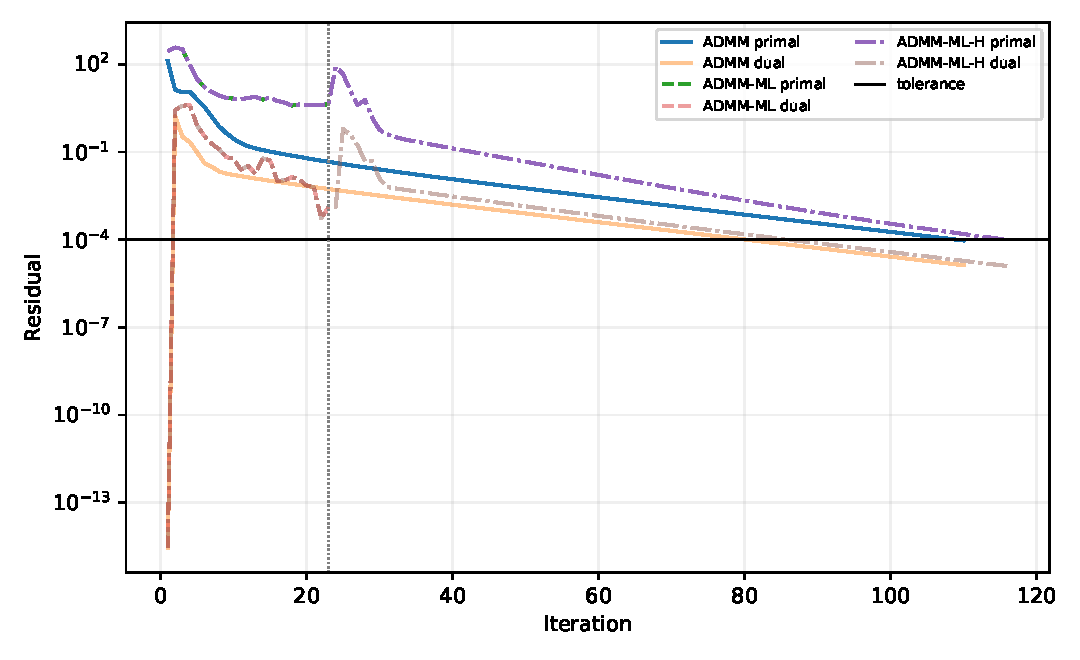
\includegraphics[width=\textwidth]{residuals_S50.pdf}
\caption{Residual histories at $S=50$, seed 99. The hybrid history includes its learned phase and exact tail. The dotted vertical line is the switch. These observations are not used to infer a contraction region.}
\label{fig:residuals}
\end{figure}

Table~\ref{tab:robustness} reports every paired exact/hybrid timing and every standalone ML terminal consensus residual. Signed speedup is $100(1-T_{\mathrm{hybrid}}/T_{\mathrm{exact}})$, so a negative value is a slowdown. At $S=20$, $\Num{HybridSlowerCountTwenty}$ of five hybrids are slower: the median signed speedup is $\Num{HybridSpeedupMedianTwenty}\%$ and the range is $\Num{HybridSpeedupMinTwenty}\%$ to $\Num{HybridSpeedupMaxTwenty}\%$. At $S=50$, $\Num{HybridFasterCountFifty}$ of five are faster, with median $\Num{HybridSpeedupMedianFifty}\%$ and range $\Num{HybridSpeedupMinFifty}\%$ to $\Num{HybridSpeedupMaxFifty}\%$. At $S=100$, $\Num{HybridFasterCountHundred}$ of five are faster, with median $\Num{HybridSpeedupMedianHundred}\%$ and range $\Num{HybridSpeedupMinHundred}\%$ to $\Num{HybridSpeedupMaxHundred}\%$. These five paired realizations per scenario count are descriptive evidence, not a confirmatory significance study or a distributional guarantee.

\begin{table}[htbp]
\centering
\caption{All 15 paired scenario realizations. Negative speedups are retained explicitly.}
\label{tab:robustness}
\small
% ===== Begin inlined file: robustness_table.tex =====
\begin{tabular}{rrrrrrr}
\toprule
$S$ & Seed & Exact (s) & Hybrid (s) & Hybrid/exact & Speedup (\%) & ML $r^K$ \\
\midrule
20 & 99 & 38.396 & 54.301 & 1.4142 & -41.42 & 2.282 \\
\midrule
20 & 100 & 38.231 & 50.285 & 1.3153 & -31.53 & 3.264 \\
\midrule
20 & 101 & 38.994 & 57.092 & 1.4641 & -46.41 & 3.772 \\
\midrule
20 & 102 & 37.975 & 47.583 & 1.2530 & -25.30 & 3.759 \\
\midrule
20 & 103 & 37.733 & 65.715 & 1.7416 & -74.16 & 3.949 \\
50 & 99 & 68.673 & 60.909 & 0.8869 & 11.31 & 4.245 \\
\midrule
50 & 100 & 64.293 & 55.613 & 0.8650 & 13.50 & 4.354 \\
\midrule
50 & 101 & 72.671 & 60.972 & 0.8390 & 16.10 & 6.513 \\
\midrule
50 & 102 & 66.693 & 56.866 & 0.8526 & 14.74 & 3.733 \\
\midrule
50 & 103 & 74.306 & 62.482 & 0.8409 & 15.91 & 3.841 \\
100 & 99 & 232.553 & 190.925 & 0.8210 & 17.90 & 4.463 \\
\midrule
100 & 100 & 239.555 & 196.291 & 0.8194 & 18.06 & 4.822 \\
\midrule
100 & 101 & 221.313 & 180.013 & 0.8134 & 18.66 & 8.181 \\
\midrule
100 & 102 & 238.049 & 190.749 & 0.8013 & 19.87 & 3.758 \\
\midrule
100 & 103 & 233.821 & 205.482 & 0.8788 & 12.12 & 4.342 \\
\bottomrule
\end{tabular}
% ===== End inlined file: robustness_table.tex =====
\end{table}

\subsection{FRL accounting}
Forward passes, FRL, consensus work, and remaining loop overhead are measured on every ML iteration. The total ML time is the measured outer wall time, not a selected sum of components. Certificate evaluation is a separate workload. There is no millisecond/second inconsistency in this table: all per-iteration entries are milliseconds and all totals are seconds. The previous $0.55$ ms versus $18{,}167.118$ ms contradiction is removed rather than reconciled from mixed logs.

\begin{table}[htbp]
\centering
\caption{Per-iteration ML component means and separately measured totals at seed 99.}
\label{tab:cost}
\footnotesize
\setlength{\tabcolsep}{4pt}
% ===== Begin inlined file: cost_table.tex =====
\begin{tabular}{rrrrrrr}
\toprule
$S$ & Forward (ms) & FRL (ms) & Consensus (ms) & Other total (s) & ML total (s) & Certificate (s) \\
\midrule
20 & 4.705 & 1.472 & 0.206 & 0.002885 & 0.118 & 0.574 \\
50 & 5.740 & 1.859 & 0.443 & 0.001244 & 0.186 & 1.430 \\
100 & 5.346 & 2.524 & 0.040 & 0.001377 & 0.183 & 3.047 \\
\bottomrule
\end{tabular}
% ===== End inlined file: cost_table.tex =====
\end{table}

\subsection{Certificate diagnostics}
Across all $\Num{RunCount}$ runs, the largest scenario-dual primal/dual spread is $\Num{MaxDualPrimalSpread}$ and the largest pinned-recourse primal/dual spread is $\Num{MaxPinnedPrimalDualSpread}$. Every computed $p_{\mathrm{low}}$ is strictly positive and every absolute gap is nonnegative. Among the $\Num{CertifiedRunCount}$ exact and hybrid runs, the maximum absolute gap is $\Num{MaxCertifiedAbsGap}$ and the maximum relative gap is $\Num{MaxCertifiedRelGapPct}\%$.

\begin{figure}[htbp]
\centering
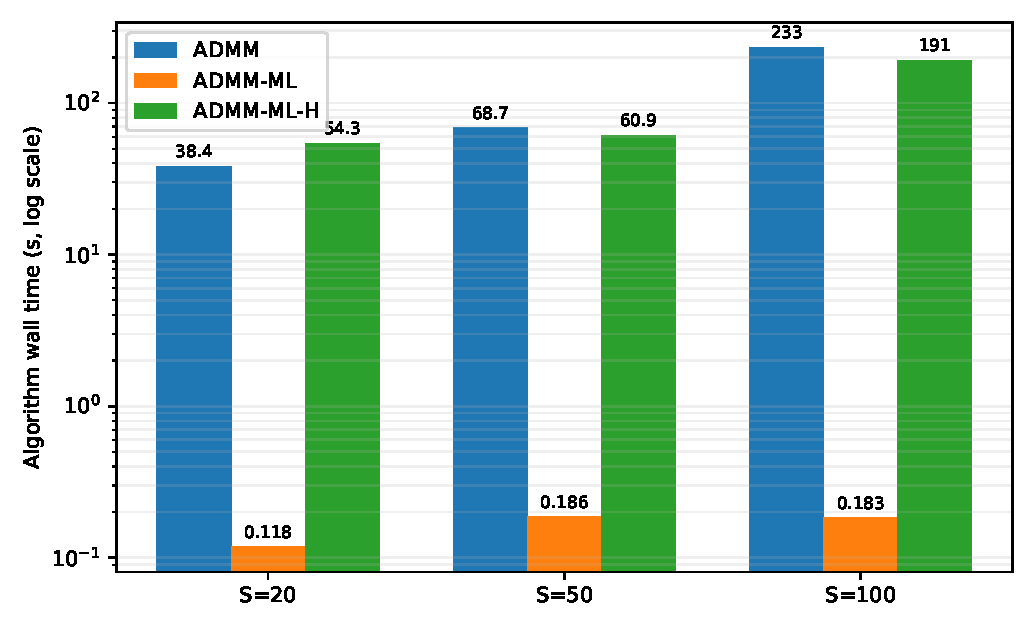
\includegraphics[width=.9\textwidth]{timings.pdf}
\caption{Measured algorithm wall times at seed 99 (logarithmic scale). Certificate evaluation is excluded here and timed separately.}
\label{fig:timings}
\end{figure}

The worst returned inner-IPM stationarity/balance residual is $\Num{WorstInnerResidual}$, the worst complementarity measure is $\Num{WorstInnerMu}$, and the largest returned iteration count is $\Num{WorstInnerIterations}$. The residual extreme occurs when the solver returns its best finite primal--dual pair instead of continuing into a singular Newton regime. We disclose these values rather than call the inner solutions machine-exact. Raw scenario dual values, primal values, slacks, terminal recourse trajectories, and all feasibility metrics are included in the reproducibility package.

Table~\ref{tab:termination} reports the actual terminal residuals and gap bounds for every run carrying a certified label, rather than only for representative instances. All $\Num{CertifiedRunCount}$ rows satisfy $r^K\leq10^{-4}$ and $s^K\leq10^{-4}$, and all relative-gap denominators $p_{\mathrm{low}}$ are strictly positive. ADMM-ML is deliberately omitted from this table because its stalled runs are not certified; its terminal consensus residuals remain visible in Tables~\ref{tab:main} and \ref{tab:robustness}, and its raw certificates remain in the release.

\begingroup
\scriptsize
\setlength{\tabcolsep}{3pt}
\setlength{\LTcapwidth}{\textwidth}
% ===== Begin inlined file: termination_table.tex =====
\begin{longtable}{rrrrrrrr}
\caption{Terminal evidence for every exact and hybrid run. Absolute gap is $V(x^K)-p_{\rm low}$; relative gaps use $p_{\rm low}>0$. The final column is the worst returned inner-QP stationarity/balance residual during that algorithm run.}\label{tab:termination}\\
\toprule
$S$ & Seed & Method & $r^K$ & $s^K$ & Abs.\ gap & Rel.\ gap (\%) & Worst inner res.\ \\
\midrule\endfirsthead
\multicolumn{8}{l}{Table \ref*{tab:termination}, continued}\\
\toprule
$S$ & Seed & Method & $r^K$ & $s^K$ & Abs.\ gap & Rel.\ gap (\%) & Worst inner res.\ \\
\midrule\endhead
\midrule\multicolumn{8}{r}{Continued on the next page}\\\endfoot
\bottomrule\endlastfoot
20 & 99 & ADMM & $9.96\times 10^{-5}$ & $7.64\times 10^{-12}$ & 0.001371 & $6.07\times 10^{-8}$ & $1.39\times 10^{-6}$ \\
20 & 99 & ADMM-ML-H & $8.04\times 10^{-5}$ & $1.52\times 10^{-9}$ & 7.291976 & $3.23\times 10^{-4}$ & $2.26\times 10^{-8}$ \\
\midrule
20 & 100 & ADMM & $9.80\times 10^{-5}$ & $9.11\times 10^{-12}$ & 0.001382 & $5.82\times 10^{-8}$ & $3.29\times 10^{-7}$ \\
20 & 100 & ADMM-ML-H & $9.84\times 10^{-5}$ & $5.58\times 10^{-11}$ & 0.511409 & $2.15\times 10^{-5}$ & $4.35\times 10^{-8}$ \\
\midrule
20 & 101 & ADMM & $9.66\times 10^{-5}$ & $6.33\times 10^{-12}$ & 0.001375 & $5.89\times 10^{-8}$ & $4.01\times 10^{-8}$ \\
20 & 101 & ADMM-ML-H & $5.97\times 10^{-5}$ & $1.31\times 10^{-9}$ & 8.089959 & $3.46\times 10^{-4}$ & $3.40\times 10^{-8}$ \\
\midrule
20 & 102 & ADMM & $9.86\times 10^{-5}$ & $4.76\times 10^{-12}$ & 0.001438 & $6.12\times 10^{-8}$ & $1.68\times 10^{-7}$ \\
20 & 102 & ADMM-ML-H & $9.84\times 10^{-5}$ & $1.07\times 10^{-8}$ & 0.004533 & $1.93\times 10^{-7}$ & $1.85\times 10^{-8}$ \\
\midrule
20 & 103 & ADMM & $9.88\times 10^{-5}$ & $7.82\times 10^{-12}$ & 0.001564 & $6.79\times 10^{-8}$ & $3.44\times 10^{-9}$ \\
20 & 103 & ADMM-ML-H & $9.99\times 10^{-5}$ & $9.64\times 10^{-10}$ & 6.186885 & $2.69\times 10^{-4}$ & $4.49\times 10^{-8}$ \\
\midrule
50 & 99 & ADMM & $9.37\times 10^{-5}$ & $1.34\times 10^{-5}$ & 0.101036 & $4.40\times 10^{-6}$ & $6.33\times 10^{-8}$ \\
50 & 99 & ADMM-ML-H & $9.84\times 10^{-5}$ & $1.25\times 10^{-5}$ & 0.093257 & $4.06\times 10^{-6}$ & $1.66\times 10^{-7}$ \\
\midrule
50 & 100 & ADMM & $9.89\times 10^{-5}$ & $1.41\times 10^{-5}$ & 0.106581 & $4.63\times 10^{-6}$ & $1.38\times 10^{-7}$ \\
50 & 100 & ADMM-ML-H & $9.97\times 10^{-5}$ & $1.29\times 10^{-5}$ & 0.096454 & $4.19\times 10^{-6}$ & $2.96\times 10^{-7}$ \\
\midrule
50 & 101 & ADMM & $9.71\times 10^{-5}$ & $1.38\times 10^{-5}$ & 0.104302 & $4.52\times 10^{-6}$ & $2.25\times 10^{-7}$ \\
50 & 101 & ADMM-ML-H & $9.33\times 10^{-5}$ & $1.29\times 10^{-5}$ & 0.094960 & $4.11\times 10^{-6}$ & $4.05\times 10^{-7}$ \\
\midrule
50 & 102 & ADMM & $9.80\times 10^{-5}$ & $1.40\times 10^{-5}$ & 0.105984 & $4.57\times 10^{-6}$ & $3.32\times 10^{-8}$ \\
50 & 102 & ADMM-ML-H & $9.84\times 10^{-5}$ & $1.29\times 10^{-5}$ & 0.095914 & $4.13\times 10^{-6}$ & $7.85\times 10^{-8}$ \\
\midrule
50 & 103 & ADMM & $9.78\times 10^{-5}$ & $1.39\times 10^{-5}$ & 0.104975 & $4.54\times 10^{-6}$ & $9.80\times 10^{-8}$ \\
50 & 103 & ADMM-ML-H & $9.95\times 10^{-5}$ & $1.32\times 10^{-5}$ & 0.096771 & $4.19\times 10^{-6}$ & $1.90\times 10^{-7}$ \\
\midrule
100 & 99 & ADMM & $9.96\times 10^{-5}$ & $2.84\times 10^{-5}$ & 0.416828 & $1.81\times 10^{-5}$ & $1.19\times 10^{-7}$ \\
100 & 99 & ADMM-ML-H & $9.87\times 10^{-5}$ & $2.74\times 10^{-5}$ & 0.411760 & $1.78\times 10^{-5}$ & $4.73\times 10^{-7}$ \\
\midrule
100 & 100 & ADMM & $9.80\times 10^{-5}$ & $2.79\times 10^{-5}$ & 0.409780 & $1.77\times 10^{-5}$ & $2.09\times 10^{-7}$ \\
100 & 100 & ADMM-ML-H & $9.71\times 10^{-5}$ & $2.70\times 10^{-5}$ & 0.403958 & $1.74\times 10^{-5}$ & $5.14\times 10^{-8}$ \\
\midrule
100 & 101 & ADMM & $9.82\times 10^{-5}$ & $2.80\times 10^{-5}$ & 0.411712 & $1.78\times 10^{-5}$ & $1.77\times 10^{-7}$ \\
100 & 101 & ADMM-ML-H & $9.70\times 10^{-5}$ & $2.70\times 10^{-5}$ & 0.405691 & $1.75\times 10^{-5}$ & $1.44\times 10^{-7}$ \\
\midrule
100 & 102 & ADMM & $9.76\times 10^{-5}$ & $2.78\times 10^{-5}$ & 0.407047 & $1.75\times 10^{-5}$ & $2.15\times 10^{-7}$ \\
100 & 102 & ADMM-ML-H & $9.91\times 10^{-5}$ & $2.76\times 10^{-5}$ & 0.412176 & $1.77\times 10^{-5}$ & $3.57\times 10^{-7}$ \\
\midrule
100 & 103 & ADMM & $9.90\times 10^{-5}$ & $2.82\times 10^{-5}$ & 0.411135 & $1.76\times 10^{-5}$ & $2.13\times 10^{-7}$ \\
100 & 103 & ADMM-ML-H & $9.85\times 10^{-5}$ & $2.75\times 10^{-5}$ & 0.404666 & $1.74\times 10^{-5}$ & $2.62\times 10^{-7}$ \\
\end{longtable}
% ===== End inlined file: termination_table.tex =====
\endgroup

\subsection{Reproducibility checks}
The release contains the complete seed-by-arm grid; no failed or unfavourable final run is dropped. For every run, a manifest records the configuration, package versions, thread settings, and SHA-256 hashes of the execution sources, checkpoint, raw NPZ, and summary. Independent verification recomputes residuals from terminal arrays, checks every scenario dual margin and absolute gap, and re-evaluates every certificate. For all 15 instances, the standalone ML history is bitwise identical to the ML phase of the corresponding hybrid run, a full learned-phase replay from the checkpoint reproduces the standalone ML state and history bitwise, and an independently recomputed exact tail reproduces the recorded terminal state and history bitwise. Dataset generation and training are also replayed bitwise for all 30 shards and for every checkpoint tensor and normalization array.

The final timing grid was freshly executed without parallel compilation, training, or visual inspection. No legacy timing is mixed into this study. $\Num{IORetryCount}$ standalone ML attempts that completed their numerical work but lost direct NPZ visibility before hashing were rerun under identical settings with stable-copy I/O handling; their failure records are retained. No seed, solver tolerance, algorithm parameter, or analysis rule was changed in response to a numerical outcome.

\begin{figure}[htbp]
\centering
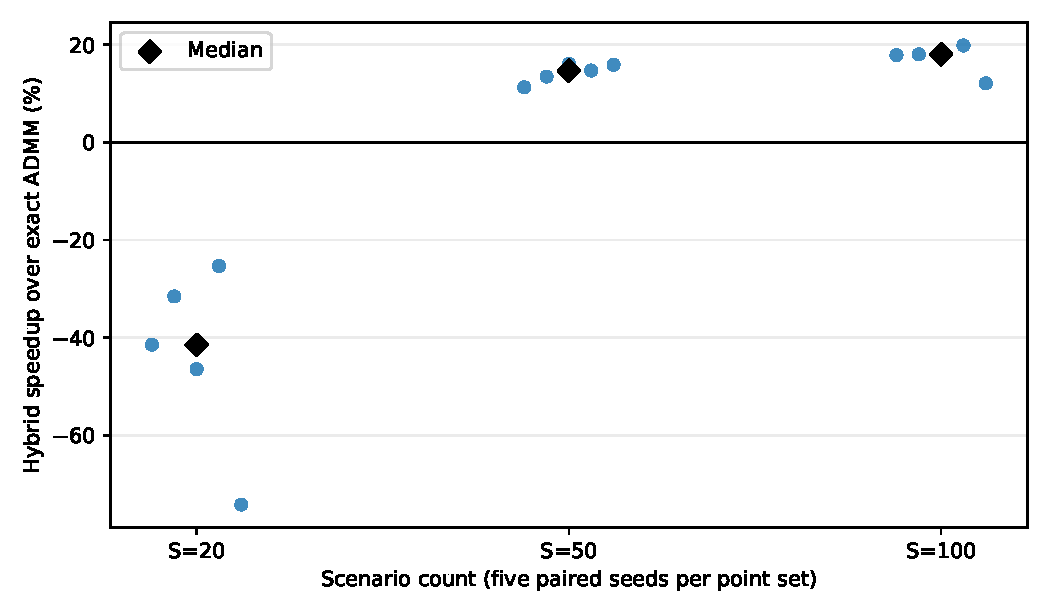
\includegraphics[width=.9\textwidth]{speedups.pdf}
\caption{Signed hybrid speedups for every paired instance. Diamonds denote medians; points above zero are faster hybrids and points below zero are slower hybrids.}
\label{fig:speedups}
\end{figure}

\section{Conclusion}
A learned initial-block update can be analyzed as an inexact DRS step, but the guarantee depends on the realized error regime. Summable errors give convergence; bounded errors give only a trapping-neighborhood bound under explicit contraction and entry hypotheses. Strong convexity with active constraints does not provide global contraction. For the constrained DC-OPF application, the defensible certified method is therefore the exact-tail hybrid, not the fixed proxy. The regenerated evidence shows why this distinction matters: the fixed proxy stalls at substantial consensus errors, while all exact and hybrid runs meet the stated residual and dual-bound checks. Certification does not imply uniform acceleration. The hybrid is slower on $\Num{HybridSlowerCountTwenty}$ of five $S=20$ instances, but faster on $\Num{HybridFasterCountFifty}$ of five $S=50$ and $\Num{HybridFasterCountHundred}$ of five $S=100$ instances in this descriptive grid. Efficiency above $S=100$, rigorous cross-topology transfer, and local linear-rate theory under separately verified regularity assumptions remain open.


\section*{Data and code availability}

The code, frozen experimental protocol, training data, trained checkpoint,
raw outputs, per-run manifests, verification scripts, and regenerated analysis
assets supporting the 45-run \texttt{strengthened-cold-v1} study are publicly
available at
\url{https://github.com/yekinishehu/learning-accelerated-admm-opf}.
The repository includes reproduction commands and SHA-256 checksum manifests
for verifying the reported residuals, certificates, tables, and figures.
The earlier twelve-run \texttt{final-cold-v1} study is not part of the
reported evidence.

% ===== End inlined file: sections/numerics.tex =====
% ===== Begin inlined file: sections/appendices.tex =====
\appendix
\section{Certificate derivations}\label{app:certificates}
\subsection{Scenario QP dual}\label{app:dual}
For one scenario, write the QP in \eqref{eq:dual}, or the analogous pinned-recourse QP, as
\begin{align*}
\min_{p,\ell,c}\quad &\frac12\sum_iw_ip_i^2+q_ip_i+\sum_t\left[C_{\mathrm{sh}}\ell_t+C_{\mathrm{cur}}c_t+\frac{\epsilon_q}{2}(\ell_t^2+c_t^2)\right]\\
\mathrm{s.t.}\quad &\sum_gp_{g,t}+\ell_t-c_t=d_t,\\
&p_i^{\min}\leq p_i\leq p_i^{\max},\qquad -R_g\leq p_{g,t}-p_{g,t-1}\leq R_g,\\
&0\leq\ell_t\leq d_t,\qquad0\leq c_t\leq W_t.
\end{align*}
Let $\nu_t$ be unrestricted balance multipliers, let $\mu_i^U,\mu_i^L\geq0$ be generation-bound multipliers, and let $\mu_{g,t}^{RU},\mu_{g,t}^{RL}\geq0$ be upper/lower ramp multipliers, and define $\Delta\mu_{g,t}=\mu_{g,t}^{RU}-\mu_{g,t}^{RL}$. Similarly, let $\mu_t^{SU},\mu_t^{SL},\mu_t^{CU},\mu_t^{CL}\geq0$ be elastic-bound multipliers. With the sign convention in which every inequality multiplier is nonnegative, minimization of the Lagrangian over $p,\ell,c$ is separable. Define
\begin{align*}
v_i^p&=q_i+\mu_i^U-\mu_i^L+\nu_{t(i)}+\Delta\mu_{g(i),t(i)}-\Delta\mu_{g(i),t(i)+1},\\
v_t^\ell&=C_{\mathrm{sh}}+\mu_t^{SU}-\mu_t^{SL}+\nu_t,\\
v_t^c&=C_{\mathrm{cur}}+\mu_t^{CU}-\mu_t^{CL}-\nu_t,
\end{align*}
where ramp terms absent at the horizon boundaries are zero. The resulting dual value is
\begin{align}
D={}&-\frac12\sum_i\frac{(v_i^p)^2}{w_i}
-\frac1{2\epsilon_q}\sum_t\left((v_t^\ell)^2+(v_t^c)^2\right)
-\sum_t\nu_td_t\nonumber\\
&-\sum_i(\mu_i^Up_i^{\max}-\mu_i^Lp_i^{\min})
-\sum_{g,t}(\mu_{g,t}^{RU}+\mu_{g,t}^{RL})R_g\nonumber\\
&-\sum_t(\mu_t^{SU}d_t+\mu_t^{CU}W_t).
\label{eq:qpdual}
\end{align}
This expression is obtained from $\min_p(v_i^pp_i+w_ip_i^2/2)=-(v_i^p)^2/(2w_i)$ and the analogous elastic minimizations. In exact real arithmetic, nonnegative bound multipliers and unrestricted $\nu$ therefore give a lower bound for every feasible primal value, irrespective of whether the computed point satisfies the stationarity equations exactly. Summing these scenario dual values and minimizing the first-stage linear term over the box $X_0$ gives the implemented evaluation of $q(\lambda)$ in \eqref{eq:dual}.

The code also records the corresponding primal QP value, scenario-by-scenario primal-minus-dual margins, and balance, box, ramp, and slack-bound violations. Any scenario margin below $-10^{-6}$ rejects the certificate. These checks do not turn binary64 arithmetic into an exact-real proof; they quantify the numerical dual evaluation actually used.

\subsection{Exact period-zero elimination for $V(x)$}\label{app:pinned}
At a pinned initial block $x$, period-zero balance is
\[
\sum_gx_g+\ell_{0,s}-c_{0,s}=D_{0,s}.
\]
If $\sum_gx_g<D_{0,s}$, optimality gives $c_{0,s}=0$ and $\ell_{0,s}=D_{0,s}-\sum_gx_g$; increasing curtailment would only increase shedding and cost. The reverse case analogously gives $\ell_{0,s}=0$ and $c_{0,s}=\sum_gx_g-D_{0,s}$. Hence
\[
\ell_{0,s}=\max(D_{0,s}-\mathbf1^\top x,0),\qquad
c_{0,s}=\max(\mathbf1^\top x-D_{0,s},0).
\]
Their generation and elastic objective contributions are then evaluated directly. Since $\sum_s\pi_s=1$, the common period-zero generation cost appears once in the expected-cost term, whereas the absolute elastic penalties are summed over all $S$ scenarios. Periods $1,\ldots,T-1$ form a reduced QP of the same class, with the first ramp window
\[
\max(p_g^{\min},x_g-R_g)\leq p_{g,1,s}\leq\min(p_g^{\max},x_g+R_g).
\]
Solving this reduced QP independently of the ADMM trajectory gives $V(x)$ in \eqref{eq:pinned}. The reported gap is the difference between this primal upper value and the scenario-dual lower value, with both primal/dual spreads retained.

\section{Numerical solver and reproducibility details}
\subsection{Batched interior-point scenario solve}
The scenario QP has a diagonal generation Hessian and tridiagonal ramp coupling. After eliminating inequality slacks, the Newton system has the form
\[
\begin{pmatrix}H&B^\top\\B&0\end{pmatrix},
\]
where $H$ consists of one tridiagonal $24\times24$ block per generator and a diagonal block for shedding and curtailment, and $B$ contains the period-balance rows. The implementation inverts the generator blocks with a batched Thomas recurrence and forms the balance Schur complement
\[
\Sigma=\sum_gH_g^{-1}+\operatorname{diag}(h_{\mathrm{sh},t}^{-1}+h_{\mathrm{cur},t}^{-1}).
\]
It solves the resulting $24\times24$ balance systems in a scenario batch and recovers the generation and elastic directions. A Mehrotra predictor--corrector determines the centering and corrector terms, with step length $0.995$ times the maximum primal/dual fraction-to-boundary steps.

Every reported ADMM scenario solve starts cold. The requested inner stopping parameters are complementarity tolerance $10^{-11}$, stationarity/balance tolerance $10^{-9}$, and at most 100 IPM iterations. The implementation tracks the best finite matched primal--dual pair. Near complementarity, the Newton systems can become numerically singular; the solver then returns that best pair rather than continuing into nonfinite arithmetic. Consequently the requested tolerances are not represented as achieved on every call: each run summary records the maximum returned residual, complementarity measure, and iteration count. This distinction is material to the numerical-certificate claim.

\subsection{Scenario profiles and exact execution protocol}
The load and wind profile vectors are
\begin{align*}
L={}&(0.67,0.63,0.60,0.59,0.60,0.64,0.74,0.83,\\
&0.90,0.95,0.97,0.96,0.95,0.95,0.93,0.94,\\
&0.99,1.00,0.99,0.96,0.91,0.83,0.75,0.70),\\
W={}&(0.62,0.65,0.67,0.68,0.66,0.62,0.55,0.47,\\
&0.40,0.34,0.30,0.28,0.27,0.28,0.31,0.35,\\
&0.40,0.45,0.50,0.54,0.57,0.60,0.61,0.62).
\end{align*}
Here $L$ is multiplied by the IEEE-118 bus loads and by a scenario scale uniform on $[0.9,1.1]$, while $W$ is multiplied by 50 MW at each wind bus. Independent AR(2) innovations use
\[
a_t=0.75a_{t-1}-0.15a_{t-2}+e_t,
\]
with zero initialization and Gaussian innovation standard deviations $0.02$ for load and $0.05$ for wind. Net load is clipped at 5\% of each bus's nominal load. Period-zero net load and wind are replaced by their scenario means. These details describe the executed parametric generator; they are not a historical-data calibration.

All final runs use Python 3.12.12, NumPy 2.2.5, and PyTorch 2.8.0, with OpenBLAS, OpenMP, MKL, and PyTorch restricted to one thread. The learned-time decomposition is
\[
T_{\mathrm{ML}}=K_{\mathrm{ml}}(\bar t_{\mathrm{fwd}}+\bar t_{\mathrm{FRL}}+\bar t_{\mathrm{cons}})+T_{\mathrm{other}},
\]
where the first three terms are sums of directly measured per-iteration components and $T_{\mathrm{other}}$ is outer wall time minus their sum. Certificate evaluation is timed separately and is excluded from algorithm speedup ratios. Offline data generation and training are reported separately and are not amortized into speedups.

\subsection{Integrity gates}
Before analysis, verification enumerates the complete scenario-count/seed/algorithm grid and rejects missing runs. For every raw run it checks SHA-256 hashes of the execution sources, checkpoint, NPZ archive, and JSON summary; recomputes terminal residuals from the saved arrays; re-evaluates every scenario and pinned-recourse certificate; and checks dual margins, nonnegative absolute gaps, positive relative-gap denominators, and both ADMM stopping tolerances. The learned phase of each hybrid run must equal its standalone ML run bitwise. Replaying the exact tail from only the saved learned endpoint must reproduce the recorded exact-tail states and residual history bitwise. Dataset and training verification separately replays all 30 shards and every checkpoint tensor and normalization array bitwise. Tables, figures, and numeric macros are generated only after these gates pass.
% ===== End inlined file: sections/appendices.tex =====

\begin{thebibliography}{99}
\bibitem{eckstein1992douglas}
J. Eckstein and D. P. Bertsekas, On the Douglas--Rachford splitting method and the proximal point algorithm for maximal monotone operators, \emph{Mathematical Programming} 55 (1992) 293--318.
\bibitem{eckstein2015understanding}
J. Eckstein and W. Yao, Understanding the convergence of the alternating direction method of multipliers: Theoretical and computational perspectives, \emph{Pacific Journal of Optimization} 11(4) (2015) 619--644.
\bibitem{liang2016convergence}
J. Liang, J. Fadili, and G. Peyr\'e, Convergence rates with inexact non-expansive operators, \emph{Mathematical Programming} 159 (2016) 403--434.
\bibitem{giselsson2017linear}
P. Giselsson and S. Boyd, Linear convergence and metric selection for Douglas--Rachford splitting and ADMM, \emph{IEEE Transactions on Automatic Control} 62(2) (2017) 532--544.
\bibitem{boyd2011distributed}
S. Boyd, N. Parikh, E. Chu, B. Peleato, and J. Eckstein, Distributed optimization and statistical learning via the alternating direction method of multipliers, \emph{Foundations and Trends in Machine Learning} 3(1) (2011) 1--122.
\bibitem{he2012convergence}
B. S. He and X. M. Yuan, On the $O(1/n)$ convergence rate of the Douglas--Rachford alternating direction method, \emph{SIAM Journal on Numerical Analysis} 50(2) (2012) 700--709.
\bibitem{liang2017local}
J. Liang, J. Fadili, and G. Peyr\'e, Local convergence properties of Douglas--Rachford and alternating direction method of multipliers, \emph{Journal of Optimization Theory and Applications} 172(3) (2017) 874--913.
\bibitem{miyato2018spectral}
T. Miyato, T. Kataoka, M. Koyama, and Y. Yoshida, Spectral normalization for generative adversarial networks, International Conference on Learning Representations, 2018.
\bibitem{zimmerman2011matpower}
R. D. Zimmerman, C. E. Murillo-S\'anchez, and R. J. Thomas, MATPOWER: Steady-state operations, planning, and analysis tools for power systems research and education, \emph{IEEE Transactions on Power Systems} 26(1) (2011) 12--19.
\bibitem{birge2011introduction}
J. R. Birge and F. Louveaux, \emph{Introduction to Stochastic Programming}, second edition, Springer, 2011.
\bibitem{shapiro2009lectures}
A. Shapiro, D. Dentcheva, and A. Ruszczy\'nski, \emph{Lectures on Stochastic Programming: Modeling and Theory}, SIAM, 2009.
\bibitem{rockafellar1991scenarios}
R. T. Rockafellar and R. J.-B. Wets, Scenarios and policy aggregation in optimization under uncertainty, \emph{Mathematics of Operations Research} 16(1) (1991) 119--147.
\bibitem{chen2022learning}
T. Chen, Y. Sun, and W. Yin, Learning to optimize: A primer and a benchmark, \emph{Journal of Machine Learning Research} 23(189) (2022) 1--59.
\bibitem{amos2023tutorial}
B. Amos, Tutorial on amortized optimization for learning to optimize over continuous domains, \emph{Foundations and Trends in Machine Learning} 16(5) (2023) 1--148.
\bibitem{sambharya2024learning}
R. Sambharya, G. Hall, B. Amos, and B. Stellato, Learning to warm-start fixed-point optimization algorithms, \emph{Journal of Machine Learning Research} 25(166) (2024) 1--46.
\end{thebibliography}
\end{document}
